\chapter{Analisis}
\label{chap:analysis}
Pada bab ini, akan dijelaskan mengenai analisis Input dan fitur perangkat lunak, Diagram pengembangan perangkat lunak, \textit{use case} dari perangkat lunak serta diagram aktifitas dari perangkat lunak.
\section{Analisis Input}
\subsection{Analisis File Excel Jadwal Mengawas Ujian}
Sub bab ini akan membahas analisis file excel yang dikeluarkan oleh TU.\\
TU FTIS mengeluarkan jadwal setiap tahunnya yang dibagikan kepada dosen FTIS. 
berikut ini contoh file excel yang dikeluarkan oleh TU. 
\begin{figure}[H]
	\centering
	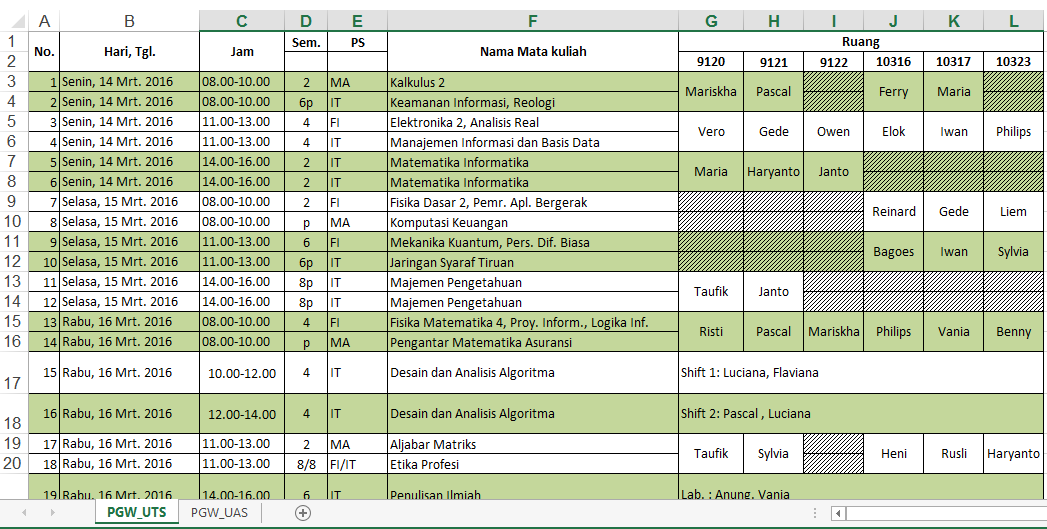
\includegraphics[scale=0.5]{Gambar/scJadwal}
	\caption{Jadwal mengawas ujian FTIS}
	\end{figure}
Dari gambar \textbf{3.1} dapat anlisa bahwa :
\begin{enumerate}
	\item Terdapat 7 kolom pada file jadwal tersebut yaitu :
		\begin{enumerate}
			\item No
			\item Hari, tanggal
			\item Jam
			\item Semester
			\item Peserta Studi
			\item Nama Mata Kuliah
			\item Ruangan (09120, 9121, 9122, 10316, 10317, 10323)
		\end{enumerate}
	\item Pada kolom semster terdapat hurf p yang menunjukan ujian tersebut merupakan mata kuliah pilihan pada semester tertentu.
	\item Pada Kolom peserta studi dapat di isi lebih dari satu jurusan ditandai dengan tanda '\textbackslash'
	\item Terdapat singkatan seperti : 
		\begin{enumerate}
			\item Tgl. pada \textit{header} merupakan singkatan dari tanggal.
			\item Sem. pada \textit{header} merupakan singkatan dari semester.
			\item PS pada \textit{header} merupakan singkatan dari peserta studi.
			\item MA pada kolom PS merupakan singkatan dari Matematika
			\item FI pada kolom PS merupakan singkatan dari Fisika
			\item IT pada kolom PS merupakan singkatan dari Informatika
			\item Mrt pada kolom Hari, Tgl. merupakan singkatan dari Maret
		\end{enumerate}
	\item kolom \textit{header} terdiri dari 2 baris, ada yang menggunakan \textit{merge}, ada juga yang dibagi menjadi 2 bagian.
	\item Kolom Ruang merupakan gabungan dari 6 kolom, dan dibawahnya tertulis nomer ruang kelas ujian.
	\item Selama satu hari jatah dosen mengawas yaitu selama 2 jam, hal itu ditandai dengan \textit{merge} 2 baris dengan nama dosen didalamnya.
	\item Ruangan yang tidak terpakai ditandai dengan warna abu bergaris - garis.
	\item Khusus untuk matakuliah pemograman tempat ujian di lab dan ada pembagian jadwal mengawas shift 1 dan shift 2.
\end{enumerate} 
 
\subsection{Analisis Fitur Perangkat Lunak}
Perangkat Lunak ini akan memiliki fitur sebagai berikut : 
	\begin{enumerate}
		\item \textit{Tool} ini dapat menerima dan membaca\textit{input} file excel jadwal mengawas ujian yang dikeluarkan TU FTIS.
		\item \textit{Tool} ini dapat mengubah file excel menjadi iCalendar.
		\item File iCalendar dapat di unduh oleh pengguna.
		\item Pengguna dapat melakukan \textit{sort} sesuai dengan nama yang di inginkan.
	\end{enumerate}
	
\section{Permodelan Tool}

Berikut diagram use case berserta skenario yang tertera pada gambar \textbf{3.2}

\begin{figure}[h]
	\centering
	\includegraphics[scale=0.5]{Gambar/useCaseJadwal}
	\caption{Diagram use case \textit{tool} konversi jadwal mengawas ujian}
	\end{figure}

\begin{enumerate}
	\item Skenario Memasukan input file excel \\
	{\renewcommand\labelitemi{}
		\begin{itemize}
			\item Deskripsi		: Kegiatan memasukan input file excel.
			\item Aktor				: Dosen
			\item Prakondisi	: -
			\item Skenario		:
				\begin{itemize}
					\item Dosen memasukan file excel mengawas ujian yang keluarkan oleh TU
				\end{itemize}
		\end{itemize}
		}
		
	\item Skenario Melakukan Sorting nama
	{\renewcommand\labelitemi{}
	\begin{itemize}
			\item Deskripsi		: Kegiatan mensorting jadwal mengawas.
			\item Aktor				: Dosen
			\item Prakondisi	: -
			\item Skenario		:
				\begin{itemize}
					\item Dosen dapat melakukan sorting nama dari jadwal ujian yang telah berupa iCal sesuai nama yang di inginkan. 
				\end{itemize}
		\end{itemize}
		}
		
		\item Skenario Mengunduh File iCal 
		{\renewcommand\labelitemi{}
		\begin{itemize}
			\item Deskripsi		: Kegiatan Mengunduh file iCal.
			\item Aktor				: Dosen 
			\item Prakondisi	: -
			\item Skenario		:
				\begin{itemize}
					\item Dosen mengunduh file iCal yang telah dikonversi oleh \textit{tool}
				\end{itemize}
		\end{itemize}
		}
		
\end{enumerate}

